\chapter{Mechanical Fasteners \& Bearings}\label{ch:fasteners}

\begin{tipbox}[When to Read This Chapter]
\textbf{Sprint~3 (CDR)}: Read when specifying fasteners in your BOM and engineering drawings. The common metric fastener sizes table is your primary reference. \textbf{Sprint~4--5}: Return to the threaded inserts section when mounting bearings or components in 3D-printed parts. The bearing selection framework applies when your project includes rotating shafts.
\end{tipbox}


\vspace{1em}

Every mechanical system is held together by fasteners and supported by bearings. Selecting the wrong bolt grade, under-torquing a critical joint, or choosing a bearing that cannot handle the load will cause your system to fail; often catastrophically and without warning. This chapter covers the fastener and bearing knowledge you need to specify these components correctly in your BOM and engineering drawings.

\vspace{1em}

\section{Threaded Fasteners}

\subsection{Bolt and Screw Anatomy}
A threaded fastener converts rotational torque into axial clamping force (preload\index{preload (bolt)}) that holds a joint together. Key parameters: \textbf{nominal diameter} (major diameter, e.g., M6 = 6\,mm), \textbf{pitch} (distance between threads; metric specifies pitch in mm; imperial uses TPI), \textbf{thread length}, and \textbf{head type} (hex, socket, flat, pan, button).

\textbf{Bolts} pass through clearance holes and clamp with a nut. \textbf{Screws} thread into a tapped hole. \textbf{Machine screws} use fine threads in tapped metal. \textbf{Self-tapping screws} form their own threads in plastic or sheet metal.

\subsection{Thread Standards}

\begin{tipbox}[Metric and Imperial Do Not Mix]
M6$\times$1.0 and 1/4-20 UNC look nearly identical (6.0\,mm vs.\ 6.35\,mm diameter). They will partially engage but strip immediately under load. Always verify with a thread gauge or package markings.
\end{tipbox}

\textbf{Unified (inch)}: UNC (Coarse) for general assembly, fewer turns, tolerant of damage. UNF (Fine) for vibration-sensitive and precision applications. \textbf{Metric (ISO)}: Designated M$d \times p$ (e.g., M6$\times$1.0). Coarse pitch is the default. Fine pitch for vibration resistance. Metric is the global standard, use for new designs unless interfacing with existing inch hardware.

\subsection{Bolt Grades and Strength}

% fig_bolt_grades.tex — SAE and ISO bolt grade markings with strength data
\begin{figure}[htbp]
\centering
\begin{tikzpicture}[
    hdr/.style={rectangle, fill=#1, text=white, minimum width=2.0cm, minimum height=0.65cm, align=center, font=\scriptsize\sffamily\bfseries},
    cell/.style={rectangle, draw=MinesBlue!30, minimum width=2.0cm, minimum height=1.2cm, align=center, font=\tiny\sffamily, inner sep=3pt, text width=1.8cm},
    grade/.style={rectangle, fill=#1!12, draw=#1!50, minimum width=2.0cm, minimum height=1.2cm, align=center, font=\scriptsize\sffamily\bfseries, text width=1.8cm, inner sep=3pt},
    mark/.style={circle, draw=#1, fill=white, minimum size=1.0cm, line width=1pt, font=\tiny\sffamily\bfseries},
]

% === SAE Section ===
\node[font=\small\sffamily\bfseries, color=MinesBlue] at (0,1.0) {SAE (Inch)};

% Column headers
\node[hdr=MinesBlue] at (0,0) {Grade};
\node[hdr=AccentTeal] at (2.2,0) {Head Mark};
\node[hdr=diagGreen] at (4.4,0) {UTS};
\node[hdr=WarnOrange] at (6.6,0) {Use};

% Grade 2
\node[grade=MinesSilver] at (0,-1.3) {Grade 2};
\node[cell] at (2.2,-1.3) {No marks};
\node[cell] at (4.4,-1.3) {74 ksi\\(510 MPa)};
\node[cell] at (6.6,-1.3) {General\\purpose};

% Grade 5
\node[grade=AccentTeal] at (0,-2.6) {Grade 5};
\node[cell] at (2.2,-2.6) {3 radial lines};
\node[cell] at (4.4,-2.6) {120 ksi\\(830 MPa)};
\node[cell] at (6.6,-2.6) {Structural\\(most common)};

% Grade 8
\node[grade=WarnOrange] at (0,-3.9) {Grade 8};
\node[cell] at (2.2,-3.9) {6 radial lines};
\node[cell] at (4.4,-3.9) {150 ksi\\(1040 MPa)};
\node[cell] at (6.6,-3.9) {High strength\\critical joints};

% === ISO Section ===
\node[font=\small\sffamily\bfseries, color=MinesBlue] at (10.5,1.0) {ISO (Metric)};

\node[hdr=MinesBlue] at (9.0,0) {Class};
\node[hdr=AccentTeal] at (11.2,0) {UTS (MPa)};
\node[hdr=diagPurple] at (13.4,0) {Yield (MPa)};

% 4.6
\node[grade=MinesSilver] at (9.0,-1.3) {4.6};
\node[cell] at (11.2,-1.3) {400};
\node[cell] at (13.4,-1.3) {240\\($4 \times 6 \times 10$)};

% 8.8
\node[grade=AccentTeal] at (9.0,-2.6) {8.8};
\node[cell] at (11.2,-2.6) {800};
\node[cell] at (13.4,-2.6) {640\\($8 \times 8 \times 10$)};

% 10.9
\node[grade=diagPurple] at (9.0,-3.9) {10.9};
\node[cell] at (11.2,-3.9) {1040};
\node[cell] at (13.4,-3.9) {940};

% 12.9
\node[grade=WarnOrange] at (9.0,-5.2) {12.9};
\node[cell] at (11.2,-5.2) {1220};
\node[cell] at (13.4,-5.2) {1100};

% Torque-preload relationship box
\node[rectangle, rounded corners=3pt, draw=MinesBlue, fill=MinesBlue!6, font=\scriptsize\sffamily, align=center, inner sep=6pt, text width=13.0cm]
    at (6.7,-6.5)
    {\textbf{Torque--Preload:} \quad $T = K \cdot F \cdot d$ \qquad
     $K = 0.20$ (dry) \quad $K = 0.15$ (lubricated) \quad $K = 0.12$ (anti-seize)\\[2pt]
     \textcolor{WarnOrange}{\textbf{90\% of torque is lost to friction}; only 10\% generates clamping force.}};

\end{tikzpicture}
\caption{SAE and ISO bolt grade markings with strength data and torque-preload relationship.}
\label{fig:grades}
\end{figure}


\textbf{SAE (inch)}: Grade~2 (no marks, 74\,ksi, general purpose), Grade~5 (3 radial lines, 120\,ksi, most common structural), Grade~8 (6 radial lines, 150\,ksi, high strength). \textbf{ISO (metric)}: Class~4.6 ($\approx$ Gr.~2), 8.8 ($\approx$ Gr.~5), 10.9 ($\approx$ Gr.~8), 12.9 (socket heads, 1220\,MPa). The first digit $\times$100 gives the UTS in MPa; the product of digits gives yield.

\begin{tipbox}[Specify the Grade]
Never list just ``M6 hex bolt'' in your BOM. Always specify: M6$\times$1.0$\times$25, Class 8.8, zinc plated. Missing the grade means the vendor ships 4.6 at half the strength.
\end{tipbox}

\subsection{Torque and Preload}
The purpose of tightening a bolt is to generate \textbf{preload} (clamping force). The torque-preload relationship:
\begin{equation}
T = K \cdot F \cdot d
\end{equation}
where $T$ = applied torque, $K$ = nut factor (0.20 dry steel, 0.15 lubricated, 0.12 anti-seize), $F$ = desired preload (typically 75\% of proof load), $d$ = nominal diameter. \textbf{90\% of applied torque is lost to friction}; only 10\% generates clamping force.

\subsection{Locking Methods}
Vibration loosens fasteners. Four reliable methods:
\begin{itemize}[nosep,leftmargin=1.5em]
\item \textbf{Nyloc nut}: nylon insert deforms around threads. One-time use per manufacturer guidance. Max 120\,\degC{}.
\item \textbf{Thread-locker}: Loctite 242 (blue, removable) for general use; 271 (red, permanent) for critical joints.
\item \textbf{Nord-Lock washers}: wedge-locking. Positive mechanical lock independent of friction. Gold standard.
\item \textbf{Safety wire}: drilled bolt heads wired in pairs. Aerospace and motorsport.
\end{itemize}

\begin{warningbox}[Split Lock Washers Are Ineffective]
Despite ubiquity, split lock washers have been shown in NASA and Junker vibration testing to provide no meaningful locking action. They flatten at low preloads and do not prevent loosening under transverse vibration. Use nyloc\index{nyloc nut} nuts, thread-locker (Loctite 242 medium-strength for removable, 271 for permanent), or Nordlock wedge-lock washers instead.
\end{warningbox}

\subsection{Non-Threaded Fasteners}
\textbf{Rivets}: permanent fasteners for sheet materials. Blind (pop) rivets install from one side. \textbf{Pins}: dowel (precision alignment), roll/spring (self-retaining), clevis (quick connect/disconnect for linkages). \textbf{Retaining rings}: external E-clips on shafts, internal in bores; inexpensive axial retention for bearings and gears. \textbf{Snap-fits}: integral plastic features; cantilever design with strain $\leq$2\% for ABS, $\leq$4\% for PP.

\begin{tipbox}[MEGN 301 Sourcing]
McMaster-Carr ships next-day to Golden and stocks every fastener here. Bolt Depot and Albany County Fasteners for bulk. For 3D-printed snap-fits, prototype in PLA, final in PETG or nylon.
\end{tipbox}

\section{Bearings}
\subsection{What Bearings Do}
Bearings support a rotating or sliding shaft while minimizing friction. Every bearing balances: \textbf{load capacity}, \textbf{speed}, \textbf{precision}, and \textbf{life}.

\subsection{Bearing Types}
\begin{figure}[htbp]\centering
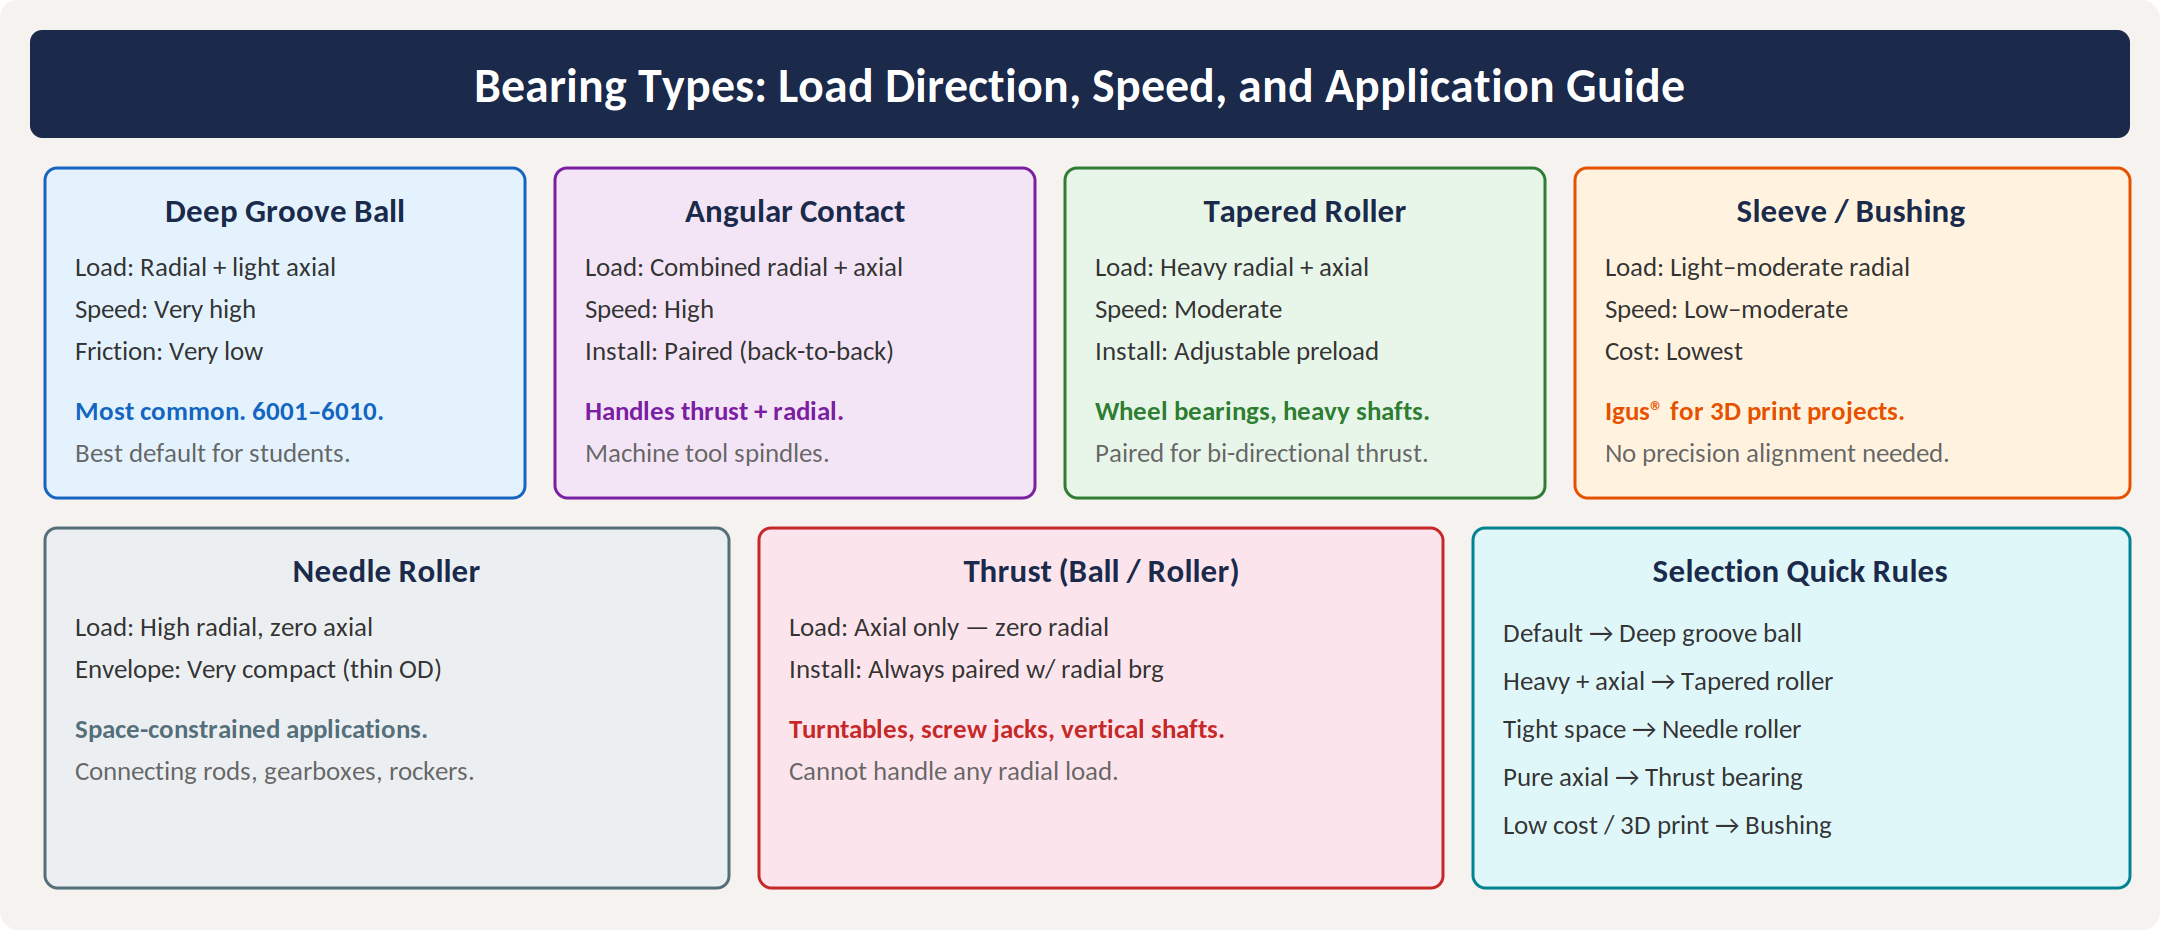
\includegraphics[width=\textwidth]{master_figs/fig_bearing_types.png}
\caption{Six bearing types with load direction, speed capability, and application guidance.}\label{fig:btypes}
\end{figure}

\textbf{Deep groove ball} (6000 series): default for students. Radial + light axial, high speed, low cost. \textbf{Angular contact}: combined radial + axial; installed in pairs. \textbf{Tapered roller}: heavy combined loads (wheel bearings). \textbf{Needle roller}: compact, high radial, zero axial. \textbf{Thrust}: axial only; always pair with a radial bearing. \textbf{Sleeve/bushing}: no rolling elements, low cost, quiet. Igus iglide\textregistered{} polymer bushings are excellent for 3D-printed housings.

\subsection{Bearing Selection}
% fig_bearing_selection.tex — Five-step bearing selection framework with failure modes
\begin{figure}[htbp]
\centering
\begin{tikzpicture}[
    step/.style={stage={#1}, text width=2.8cm, minimum height=1.4cm, font=\scriptsize\sffamily\bfseries},
    num/.style={circle, fill=#1, text=white, font=\scriptsize\sffamily\bfseries, minimum size=0.5cm, inner sep=0pt},
    fail/.style={rectangle, rounded corners=2pt, draw=diagRed!70, fill=diagRed!6, text width=2.4cm, minimum height=0.7cm, align=center, font=\tiny\sffamily, inner sep=3pt},
    conn/.style={flow={MinesBlue!70}, line width=1.2pt},
]

% Five steps in a row
\node[step=MinesBlue] (s1) at (0,0) {Load Type\\and Magnitude\\Calculate $P$};
\node[step=AccentTeal] (s2) at (3.4,0) {Speed\\Check limiting\\RPM};
\node[step=diagPurple] (s3) at (6.8,0) {Space\\Bore \& OD\\constraints};
\node[step=WarnOrange] (s4) at (10.2,0) {Life\\$L_{10}$ calculation};
\node[step=diagGreen] (s5) at (13.6,0) {Mounting\\Press fit,\\retaining ring};

% Step numbers
\node[num=MinesBlue, above left=0.1cm and 0.1cm of s1.north west] {1};
\node[num=AccentTeal, above left=0.1cm and 0.1cm of s2.north west] {2};
\node[num=diagPurple, above left=0.1cm and 0.1cm of s3.north west] {3};
\node[num=WarnOrange, above left=0.1cm and 0.1cm of s4.north west] {4};
\node[num=diagGreen, above left=0.1cm and 0.1cm of s5.north west] {5};

% Arrows between steps
\draw[conn] (s1) -- (s2);
\draw[conn] (s2) -- (s3);
\draw[conn] (s3) -- (s4);
\draw[conn] (s4) -- (s5);

% Life equation
\node[rectangle, rounded corners=2pt, draw=MinesBlue, fill=MinesBlue!6, font=\tiny\sffamily, align=center, inner sep=4pt]
    at (10.2,-1.8)
    {$L_{10} = \left(\frac{C}{P}\right)^3 \times \frac{10^6}{60n}$ hrs};

% Failure modes section
\node[font=\small\sffamily\bfseries, color=diagRed] at (6.8,-3.0) {Common Failure Modes};

\node[fail] (f1) at (1.7,-4.0) {\textbf{Brinelling}\\Static overload\\dents raceway};
\node[fail] (f2) at (5.1,-4.0) {\textbf{Spalling}\\Fatigue flaking\\(normal end-of-life)};
\node[fail] (f3) at (8.5,-4.0) {\textbf{Contamination}\\Particles accelerate\\wear $10\times$};
\node[fail] (f4) at (11.9,-4.0) {\textbf{Misalignment}\\Angular error\\causes edge loading};

\end{tikzpicture}
\caption{Five-step bearing selection framework with common failure modes.}
\label{fig:bsel}
\end{figure}


Five steps: (1) \textbf{Load type and magnitude}; calculate equivalent dynamic load $P$. (2) \textbf{Speed}; check limiting RPM. (3) \textbf{Space}; bore and OD constraints. (4) \textbf{Life}; $L_{10} = (C/P)^p \times 10^6 / (60n)$ hours. (5) \textbf{Mounting}; press fit, retaining ring, adhesive.

\begin{tipbox}[Bearing Sizing for Student Projects]
(1) Select shaft diameter. (2) Look up matching bearing (8\,mm shaft $\to$ 608-2RS, \$2). (3) Verify $C \geq 3\times$ max load. (4) Order 2RS (sealed) variant. Done.
\end{tipbox}

\subsection{Mounting Bearings}
\textbf{Press fit}: bore interference fit on shaft (0.005--0.015\,mm). Use an arbor press; press only on the fitted ring.

\begin{tipbox}[Mounting Bearings in 3D Prints]
FDM tolerance $\pm$0.2--0.3\,mm. For bearing pockets: design 0.1--0.2\,mm undersize and ream to fit, or 0.05\,mm oversize with retaining compound (Loctite 638). Always test-fit with a prototype print.
\end{tipbox}

\begin{warningbox}[Never Hammer a Bearing]
Striking a bearing transmits shock through rolling elements, creating brinelling dents. These cause vibration, noise, and premature failure. Always use an arbor press or soft-jaw vise.
\end{warningbox}

\subsection{Failure Modes}
\textbf{Brinelling}: static overload dents raceway. \textbf{Spalling}: fatigue flaking (normal end-of-life). \textbf{Contamination}: particles accelerate wear $10\times$; use sealed (2RS) bearings. \textbf{Misalignment}: angular error causes edge loading.


\subsection{Thread Engagement Table}
\begin{table}[htbp]\centering\small
\begin{tabularx}{\textwidth}{l c c X}
\toprule
\textbf{Material} & \textbf{Min Engagement} & \textbf{Preferred} & \textbf{Notes} \\
\midrule
Steel & 1.0$d$ & 1.5$d$ & Standard for structural joints \\
Aluminum & 1.5$d$ & 2.0$d$ & Softer threads require more engagement \\
Cast iron & 1.5$d$ & 2.0$d$ & Brittle; threads can crack if overtorqued \\
Plastic (ABS) & 2.0$d$ & 2.5$d$ & Use coarse thread; consider threaded insert\index{threaded insert} \\
Brass & 1.5$d$ & 2.0$d$ & Avoid for high-torque applications \\
\bottomrule
\end{tabularx}
\caption{Minimum thread engagement\index{thread engagement} by material.}
\end{table}

\subsection{Threaded Inserts for 3D-Printed Parts}
Direct threading into FDM plastic is unreliable; the threads strip under moderate torque. Three better options: \textbf{Heat-set brass inserts} (pressed in with a soldering iron; strongest, most professional), \textbf{press-fit inserts} (pushed into undersized holes; adequate for light loads), and \textbf{captive nuts} (hex nut trapped in a designed pocket during printing). Heat-set inserts (McMaster \#94180A series) are the recommended solution for MEGN~301 projects.

\subsection{Bolt Selection Checklist}
\begin{enumerate}[nosep,leftmargin=1.5em]
\item Determine joint loads (tension, shear, or combined).
\item Select thread standard (metric for new designs).
\item Select grade/class based on load with $\geq$2$\times$ safety factor.
\item Size diameter from shear/tension calculations.
\item Determine length: grip length + nut + washer + 2--3 exposed threads.
\item Specify head type based on tool access and flush requirements.
\item Specify locking method based on vibration environment.
\item Calculate and specify torque value.
\item Add all details to BOM entry.
\end{enumerate}

\section{Design Rules of Thumb}
\begin{enumerate}[leftmargin=1.5em]
\item Thread engagement: min 1.5$d$ in steel, 2$d$ in aluminum, 2.5$d$ in plastic.
\item Bolt spacing: min 3$d$ center-to-center, 2$d$ from edge.
\item Inner ring press fit to shaft; outer ring sliding fit to housing (rotating-shaft case).
\item Always specify grade, material, finish, and torque in assembly documentation.
\end{enumerate}


\begin{keyconceptbox}[Requirements Mapping: From Fastener Specs to Shall-Statements]
Mechanical joining generates system requirements:
\begin{itemize}[nosep,leftmargin=1.5em]
\item ``Vibration environment (field deployment)'' $\to$ MECH-REQ: All structural fasteners shall use positive locking (nyloc, thread-locker, or Nord-Lock). Split washers shall not be used.
\item ``Enclosure opens for maintenance'' $\to$ MECH-REQ: Enclosure fasteners shall be captive (retained in the cover after removal) and require only a \#2 Phillips driver.
\item ``Shaft supports 50\,N radial load at 1500\,RPM'' $\to$ BRG-REQ: Shaft bearing shall have $L_{10} \geq 5000$\,hrs at the specified load and speed. Bearing type: deep-groove ball, sealed (2RS).
\end{itemize}
\end{keyconceptbox}

\section{Threaded Fastener Design}
\subsection{Bolt Sizing}
The primary design criterion for a bolted joint is the clamping force. The bolt must provide sufficient clamping force to prevent joint separation under the maximum expected external load, plus a safety factor. The clamping force is related to the tightening torque by:
\begin{equation}
T = K \cdot d \cdot F_i
\end{equation}
where $T$ is the torque, $K$ is the nut factor (approximately 0.2 for dry steel, 0.15 for lubricated), $d$ is the nominal bolt diameter, and $F_i$ is the initial clamping force (preload). For the joint to remain clamped under external load $F_{\text{ext}}$: $F_i > F_{\text{ext}} / (1 - C)$ where $C$ is the joint stiffness ratio (typically 0.1--0.3 for metal-on-metal joints).

\subsection{Thread Engagement}
The minimum thread engagement length to develop full bolt strength: for steel bolts in steel: $L_e \geq 1.0d$ (one diameter). For steel bolts in aluminum: $L_e \geq 1.5d$ (the aluminum threads are weaker). For steel bolts in plastic: $L_e \geq 2.5d$ or use threaded inserts (Heli-Coils).

\subsection{Thread Locking}
Under vibration, threaded fasteners can loosen. Prevention methods: (1) \textbf{Nylon-insert lock nuts} (Nyloc): a nylon collar in the nut provides friction that resists loosening. Effective, low cost, one-time use per manufacturer guidance. (2) \textbf{Thread-locking adhesive} (Loctite): blue (242) for medium strength (removable with hand tools), red (271) for permanent (requires heat to remove). (3) \textbf{Split lock washers}: limited effectiveness; largely replaced by Nordlock wedge-locking washers. (4) \textbf{Safety wire}: for high-vibration aerospace applications (drilling the bolt head and wiring to an adjacent bolt).

\section{Bearing Selection and Installation}
\subsection{Bearing Sizing}
Bearings are sized by their rated life, which depends on the applied load:
\begin{equation}
L_{10} = \left(\frac{C}{P}\right)^3 \text{ (ball bearings\index{ball bearing})} \qquad L_{10} = \left(\frac{C}{P}\right)^{10/3} \text{ (roller bearings\index{roller bearing})}
\end{equation}
where $L_{10}$ is the life in millions of revolutions (90\% survival probability), $C$ is the basic dynamic load rating (from the catalog), and $P$ is the equivalent dynamic load. For a 608 bearing ($C = 3.45$\,kN) under 100\,N radial load: $L_{10} = (3450/100)^3 = 41{,}063$ million revolutions. At 1000\,RPM: this is 683,000 hours, far exceeding any project lifetime. Bearings in MEGN~301 projects are almost never load-limited; select based on size, availability, and cost.

\subsection{Bearing Installation}
Press the bearing onto the shaft by applying force to the inner ring (not the outer ring). For housing installation: press on the outer ring. Never apply force through the rolling elements (this creates dents in the raceways, called brinelling, which causes noise and premature failure). Use an arbor press with a properly sized tube that contacts only the ring being pressed. For light press fits: use a dead-blow hammer with a bearing installation tool. Apply a thin film of oil to the shaft and housing bore before installation.

\section{Design for Assembly (DfA)}
\textbf{Minimize part count}: every part that can be eliminated saves assembly time, reduces potential failure points, and simplifies inventory. Challenge every part: can it be combined with an adjacent part? Can its function be achieved by a feature of another part?

\textbf{Design for top-down assembly}: parts should assemble from one direction (typically gravity-assisted, top-down). Avoid requiring the assembler to flip, rotate, or hold the assembly in unstable orientations.

\textbf{Self-locating features}: use chamfers, tapers, and guide pins to align parts during assembly. A part that can only be assembled one way (poka-yoke) eliminates assembly errors.

\textbf{Standard hardware}: use the minimum number of fastener types and sizes. Ideally, one M3 screw size for all internal fasteners and one M5 for external/structural fasteners. This minimizes the tool kit and eliminates wrong-fastener errors.
\section{Fastener Material Selection}
\textbf{Low-carbon steel (Grade 2/SAE J429)}: the most common and cheapest fastener material. Tensile strength $\sim$510\,MPa. Adequate for most non-critical applications. Usually zinc-plated for corrosion resistance (adequate for indoor use; inadequate for outdoor or wet environments).

\textbf{Medium-carbon steel (Grade 5/SAE J429)}: quenched and tempered. Tensile strength $\sim$830\,MPa. Standard for automotive and structural applications. Three radial marks on the hex head identify Grade~5.

\textbf{Alloy steel (Grade 8/SAE J429)}: highest standard grade. Tensile strength $\sim$1040\,MPa. Six radial marks. Use when high clamping force is needed in a small bolt (e.g., mounting a motor that generates high vibration).

\textbf{Stainless steel (A2/304 and A4/316)}: corrosion resistant but lower strength than Grade 5 ($\sim$700\,MPa for A2). Non-magnetic (mostly). Use in wet environments, food equipment, and medical devices. Galling risk: stainless-on-stainless threads can cold-weld during tightening. Always use anti-seize compound (nickel-based: Permatex Nickel Anti-Seize or Loctite LB~8023) on stainless fasteners.

\textbf{Nylon and other polymers}: electrically insulating, non-marring, lightweight. Very low strength ($\sim$70\,MPa). Use for PCB mounting, panel retention, and applications where electrical isolation is required.

\section{Metric vs.\ Imperial Fasteners}
MEGN~301 uses metric fasteners exclusively (M2, M2.5, M3, M4, M5, M6, M8). Key dimensions:

\begin{itemize}[nosep,leftmargin=1.5em]
\item M3: 3.0\,mm diameter, 0.5\,mm pitch, 2.5\,mm hex socket (most common for electronics/small mechanisms)
\item M4: 4.0\,mm, 0.7\,mm pitch, 3.0\,mm hex
\item M5: 5.0\,mm, 0.8\,mm pitch, 4.0\,mm hex (structural connections)
\item M6: 6.0\,mm, 1.0\,mm pitch, 5.0\,mm hex
\end{itemize}

\textbf{Never mix metric and imperial fasteners in the same assembly}. They are not interchangeable: an M6 bolt ($6.0\times 1.0$\,mm) will cross-thread into a 1/4-20 UNC hole ($6.35\times 1.27$\,mm), destroying both threads.

\section{Threaded Insert Technology}
When bolting into soft materials (3D-printed plastic, wood, aluminum sheet), direct threading provides insufficient strength and wear resistance. Threaded inserts solve this:

\textbf{Heat-set inserts} (brass, knurled): heated with a soldering iron and pressed into a slightly undersized hole in thermoplastic. The plastic melts around the knurls and re-solidifies, creating a permanent, high-pullout-strength metal thread. Standard for 3D-printed enclosures. Use an insert tip on the soldering iron for consistent installation.

\textbf{Heli-Coil inserts} (stainless steel wire coils): installed into a tapped hole of the correct Heli-Coil drill and tap size. Create a wear-resistant thread in aluminum, magnesium, and other soft metals. Standard for aerospace and automotive repair of stripped threads.

\textbf{Press-in inserts} (brass, steel): pressed into a hole with an arbor press. The knurled exterior grips the surrounding material. Used in plastic injection-molded parts and machined assemblies.

\section{Adhesive Bonding}
When mechanical fasteners are impractical (thin materials, aesthetic requirements, vibration-sensitive joints), adhesives provide an alternative:

\textbf{Cyanoacrylate (CA, ``super glue'')}: fast cure (seconds), high shear strength ($\sim$20\,MPa), brittle. Good for: bonding small plastic parts, tacking components during assembly, and strain gauge installation. Poor gap-filling; requires intimate contact.

\textbf{Epoxy (two-part)}: slow cure (5 minutes to 24 hours depending on formulation), very high strength ($\sim$35\,MPa shear, $\sim$70\,MPa tensile), excellent gap-filling, chemical resistant. Standard structural adhesive. 5-minute epoxy is convenient but weaker than 24-hour types.

\textbf{Silicone (RTV)}: flexible, waterproof, temperature resistant ($-60$ to $+200$\,\degC{}). Low strength ($\sim$2\,MPa). Use for sealing, vibration isolation, and potting electronics. Not a structural adhesive.

\textbf{Thread-locking adhesive} (Loctite): applied to bolt threads to prevent loosening. Blue (242): medium strength, removable with hand tools. Red (271): permanent, requires heat ($\sim$250\,\degC{}) to remove. Purple (222): low strength, for small screws (M2--M6) that must be removable.

\begin{warningbox}[Adhesive Surface Preparation]
Adhesive strength depends critically on surface cleanliness. Always clean bonding surfaces with isopropanol (IPA) before applying adhesive. For metals: abrade lightly with 320-grit sandpaper, then clean with IPA. For plastics: IPA wipe only (abrasion can create micro-cracks that weaken the joint). For 3D-printed PLA: adhesion is poor on smooth surfaces; lightly sand to create mechanical interlock.
\end{warningbox}

\begin{quickrefbox}[Quick Reference: Common Metric Fastener Sizes]
\begin{table}[H]\centering\small
\begin{tabularx}{\linewidth}{c c c c c X}
\toprule
\textbf{Size} & \textbf{Pitch} & \textbf{Clearance} & \textbf{Tap Drill} & \textbf{Torque\textsuperscript{a}} & \textbf{Typical Use} \\
\midrule
M2 & 0.4\,mm & 2.4\,mm & 1.6\,mm & 0.2\,N$\cdot$m & Electronics, PCB standoffs \\
M3 & 0.5\,mm & 3.4\,mm & 2.5\,mm & 0.6\,N$\cdot$m & Small brackets, sensor mounts \\
M4 & 0.7\,mm & 4.5\,mm & 3.3\,mm & 1.5\,N$\cdot$m & General assembly, motor mounts \\
M5 & 0.8\,mm & 5.5\,mm & 4.2\,mm & 3.0\,N$\cdot$m & Medium structural, T-slot extrusion \\
M6 & 1.0\,mm & 6.6\,mm & 5.0\,mm & 5.5\,N$\cdot$m & Heavy structural, brackets \\
M8 & 1.25\,mm & 9.0\,mm & 6.8\,mm & 14\,N$\cdot$m & High-load joints, flanges \\
\bottomrule
\multicolumn{6}{l}{\textsuperscript{a}Class 8.8 bolt, dry ($K=0.20$). Lubricated: multiply by 0.75.}
\end{tabularx}
\end{table}
\end{quickrefbox}

\section{Practice Questions}
\begin{enumerate}[leftmargin=1.5em]
\item Your design uses an M8$\times$1.25 bolt in tapped aluminum. Minimum thread engagement depth? If limited to 10\,mm, is this sufficient?
\item A joint experiences severe vibration. Compare nyloc, Loctite 242, and Nord-Lock. Recommend one.
\item Your BOM lists ``1/4-20 bolt, qty 12'' with no other info. What is wrong? Rewrite it properly.
\item Select a bearing for an 8\,mm shaft at 3000\,RPM with 50\,N radial load. Specify designation, type, expected life.
\item A teammate suggests press-fitting bearings into PLA housings. Identify two problems and propose solutions.
\item Belt-driven stage idler pulley bearings grind after one week. Likely causes and diagnosis?
\item An M6 Class 8.8 bolt has proof load $\approx$16.3\,kN. Calculate torque for 75\% proof load preload ($K=0.20$).
\end{enumerate}

\subsection{Answers}
\begin{enumerate}[leftmargin=1.5em]
\item Min = 2$\times$8\,mm = 16\,mm for aluminum. 10\,mm = 1.25$d$; insufficient. Use through-bolt with nut, Heli-Coil insert, or thicker boss.
\item Nord-Lock for severe vibration with frequent disassembly. Loctite 271 (red) for permanent assembly. Nyloc for general use.
\item Missing: grade, head type, length, material/finish, torque. Correct: ``1/4-20 UNC $\times$ 1.00\,in hex cap, SAE Grade 5, zinc, qty 12. Torque: 8.0\,ft-lb with Loctite 242.''
\item 608-2RS: 8\,mm bore, 22\,mm OD. $C = 3.45$\,kN, $P = 0.05$\,kN. $L_{10} = (3.45/0.05)^3 \times 10^6/(60 \times 3000) = 918{,}000$\,hrs.
\item PLA: low HDT ($\sim$60\,\degC{}), creeps under load $\to$ pocket enlarges. Tolerance $\pm$0.2\,mm makes press fit unreliable. Fix: use PETG/nylon, ream pocket, or use retaining compound.
\item Contamination, misalignment, or open (unsealed) bearings. Diagnosis: spin by hand (gritty = contamination), check housing alignment, inspect seals. Replace with 2RS type.
\item $F = 0.75 \times 16{,}300 = 12{,}225$\,N. $T = 0.20 \times 12{,}225 \times 0.006 = 14.7$\,N$\cdot$m.
\end{enumerate}


